\chapter{Background}
\label{cha:relatedwork}

In this section, the global system known as \emph{devices cloud} will be first detailed. Afterwards, the different possible technologies that could be used in this thesis will be introduced. Finally, an overview of the different researches and studies that have been previously performed will be given.
 
\section{The Devices Cloud}
Integrating the requirements defined in the Introduction to a more detailed view of the global system, the Figure \ref{fig:design_complete} of the \emph{devices cloud} architecture . Of course, only the information relevant for this thesis is depicted.

\begin{figure}[!ht]
	\centering
	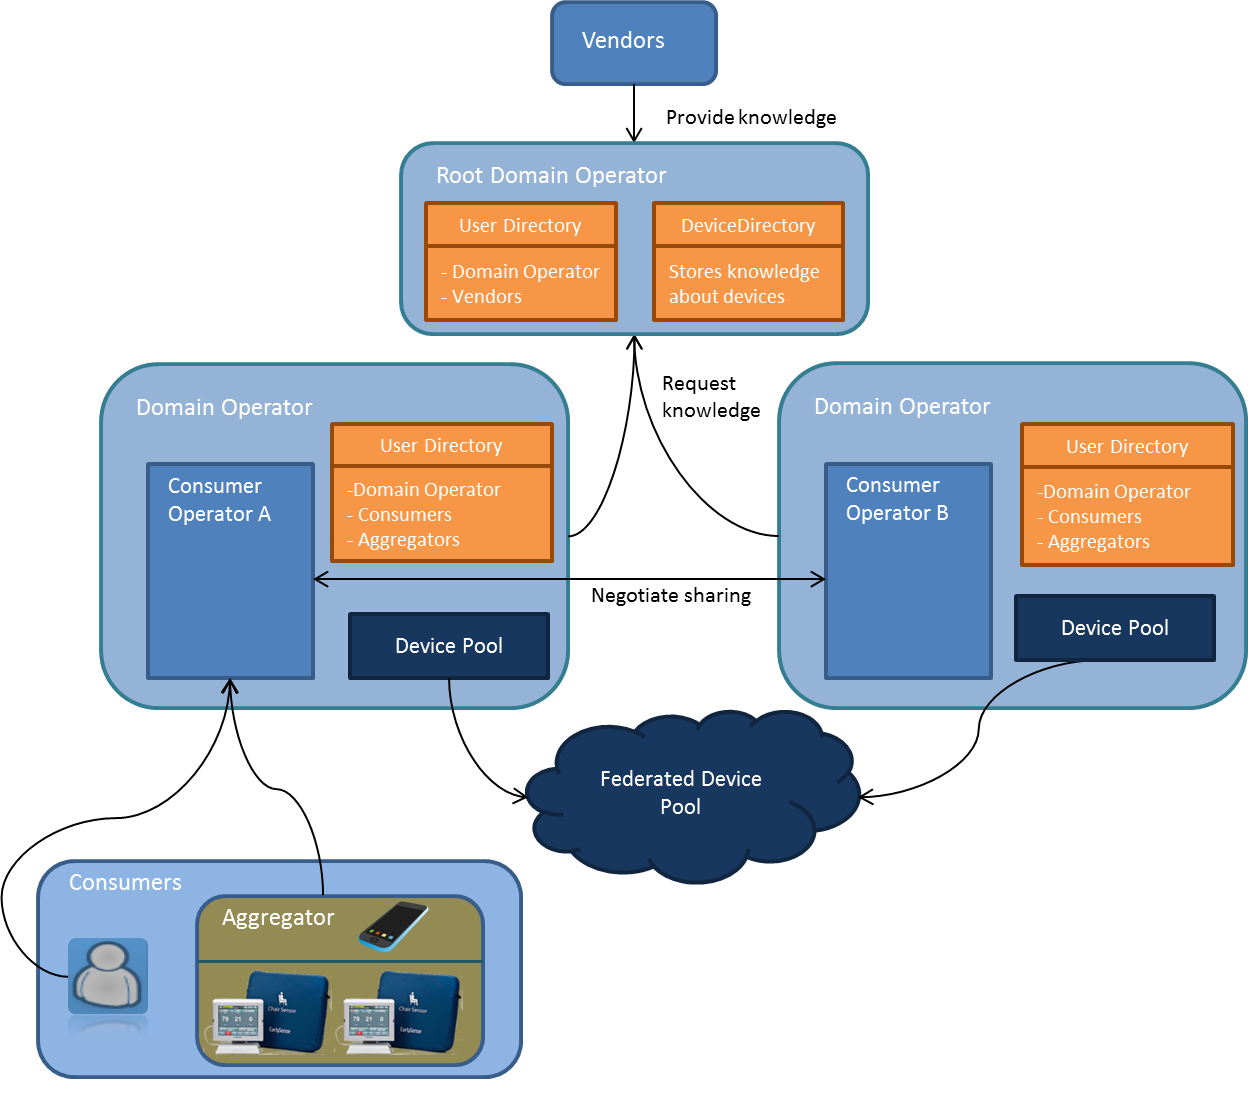
\includegraphics[scale=0.3]{images/design_complete}
	\caption{Detailed Architecture of the Devices Cloud}
	\label{fig:design_complete}
\end{figure}

Every Domain Operator maintain a User Directory and a Device Directory. The earlier is used to authenticate and authorize every entities that can be. The latter is used to store the information about every device operated by the operator.

The Device Directory is particularly important for authorization purposes, because it stores knowledge like the Device Owner and Device Operator for every device. As explained in the Introduction, those two roles are the only ones that are authorized, for example, to revoke a device's access. 

In the framework, the Device Directory could then be compared to the authorization server in the sense that it can map an entity with roles.

This Device Directory has a public interface, the Device Pool, containing the devices they operate. This Device Pool contains only the information that an end customer can see in order to choose which devices he wants to have access to. The different device pools contribute then to a Federated Device Pool, containing all devices available to the customers. Those, when registered to their Domain Operator, can have access to this Federated Pool. Of course, the different pools of devices must be synchronized, but it will not be explained in this thesis.

When a customer has chosen which devices he wants to read the data from, he uses an aggregator, most likely its mobile phone, to integrate the different devices. The authentication of the different actors is first performed (intra Operators, between Customer and Domain Operator, ...), the required data (like drivers) is then retrieved from the Domain Operators or Root Domain Operator and the data from of the device can eventually be read.

 \subsection{Entities}
 In \citetitle{reference_thesis}, four main characteristics have been defined for the entities present in the \emph{device cloud}:
 
% \begin{table}[!ht]
% 	\caption{Type of Entities in the Device Cloud}
%	 \centering
	 \def\arraystretch{1.5}
%	 \setlength{\extrarowheight}{15pt}
	 \begin{longtable}{|m{\textwidth}|}
	 	\caption{Type of Entities in the Device Cloud} \\
	 	\hline
	 	\rowcolor{Gray}\textcolor{white}{\textbf{  Entities Characteristics}}
	 	\\ \hline

		
	 	\pbox{\linewidth}{
	 		\vspace*{10pt}
		 	 \textbf{Attachment Entity:} \\
	 		 An attachment refers to any kind of resource usually stored on the file system (e.g.	a picture or a binary). Attachment Entities can have several attachments.
	 		}
	 		\\ \hline
	 	
	 	\pbox{\linewidth}{
	 		\vspace*{10pt}
	 		\textbf{Configurable Entity:} \\
	 		A configurable entity holds a set of configuration entries expressed as key-value pairs. Each entry again is backed by the global entity definition (in the Root Domain). This means, that each local copy of an entity can have two virtual sets of configuration entries.
	 	} \\
 	\hline
 		\pbox{\linewidth}{
 			\vspace*{10pt}
 			\textbf{Location Tagged Entity:} \\
 			An entity whose location can be monitored. This can be an important parameter
 			when having to decide about competing device access re quests or requests to devices
 			that are already provisioned. 
 		} \\
 		\hline
 		\pbox{\linewidth}{
 			\vspace*{10pt}
 			\textbf{Principal Entity:} \\
 			A Principal Entity is an entity that can be authenticated by the User Directory using its EntityID and some kind of security credentials (e.g. certificate or password).
 			Examples are Consumer Operators, Consumers, Aggregators or Vendor. 
 		} \\
 		\hline
 \end{longtable}
 
 in this thesis, the focus will be put on Principal Entities, since it's the most relevant characteristic when designing an authentication framework. However, an entities can have several characteristics at the same time. Every type of entity must then be taken into consideration.

% \end{table}
 



\section{Authentication}
\subsection{Authentication from symmetric key}
\subsection{Authentication from asymmetric keys}
\subsection{Authentication from one-way function}
\subsection{Federated Identity Management}
\subsubsection{Kerberos}
\subsubsection{SAML}
\subsubsection{OpenId}
\subsubsection{OpenId Connect}

\section{Related work}